% Options for packages loaded elsewhere
\PassOptionsToPackage{unicode}{hyperref}
\PassOptionsToPackage{hyphens}{url}
%
\documentclass[
  11pt,
]{article}
\usepackage{amsmath,amssymb}
\usepackage{iftex}
\ifPDFTeX
  \usepackage[T1]{fontenc}
  \usepackage[utf8]{inputenc}
  \usepackage{textcomp} % provide euro and other symbols
\else % if luatex or xetex
  \usepackage{unicode-math} % this also loads fontspec
  \defaultfontfeatures{Scale=MatchLowercase}
  \defaultfontfeatures[\rmfamily]{Ligatures=TeX,Scale=1}
\fi
\usepackage{lmodern}
\ifPDFTeX\else
  % xetex/luatex font selection
\fi
% Use upquote if available, for straight quotes in verbatim environments
\IfFileExists{upquote.sty}{\usepackage{upquote}}{}
\IfFileExists{microtype.sty}{% use microtype if available
  \usepackage[]{microtype}
  \UseMicrotypeSet[protrusion]{basicmath} % disable protrusion for tt fonts
}{}
\makeatletter
\@ifundefined{KOMAClassName}{% if non-KOMA class
  \IfFileExists{parskip.sty}{%
    \usepackage{parskip}
  }{% else
    \setlength{\parindent}{0pt}
    \setlength{\parskip}{6pt plus 2pt minus 1pt}}
}{% if KOMA class
  \KOMAoptions{parskip=half}}
\makeatother
\usepackage{xcolor}
\usepackage[margin=2.5cm]{geometry}
\usepackage{color}
\usepackage{fancyvrb}
\usepackage{fvextra}
\newcommand{\VerbBar}{|}
\newcommand{\VERB}{\Verb[commandchars=\\\{\}]}
\DefineVerbatimEnvironment{Highlighting}{Verbatim}{commandchars=\\\{\},breaklines=true,breakanywhere=true,fontsize=\small}
\DefineVerbatimEnvironment{verbatim}{Verbatim}{breaklines=true,breakanywhere=true,fontsize=\footnotesize,breaksymbol={}}
\newenvironment{Shaded}{\vspace{4pt}}{\vspace{4pt}}
\newcommand{\AlertTok}[1]{\textcolor[rgb]{1.00,0.00,0.00}{\textbf{#1}}}
\newcommand{\AnnotationTok}[1]{\textcolor[rgb]{0.38,0.63,0.69}{\textbf{\textit{#1}}}}
\newcommand{\AttributeTok}[1]{\textcolor[rgb]{0.49,0.56,0.16}{#1}}
\newcommand{\BaseNTok}[1]{\textcolor[rgb]{0.25,0.63,0.44}{#1}}
\newcommand{\BuiltInTok}[1]{\textcolor[rgb]{0.00,0.50,0.00}{#1}}
\newcommand{\CharTok}[1]{\textcolor[rgb]{0.25,0.44,0.63}{#1}}
\newcommand{\CommentTok}[1]{\textcolor[rgb]{0.38,0.63,0.69}{\textit{#1}}}
\newcommand{\CommentVarTok}[1]{\textcolor[rgb]{0.38,0.63,0.69}{\textbf{\textit{#1}}}}
\newcommand{\ConstantTok}[1]{\textcolor[rgb]{0.53,0.00,0.00}{#1}}
\newcommand{\ControlFlowTok}[1]{\textcolor[rgb]{0.00,0.44,0.13}{\textbf{#1}}}
\newcommand{\DataTypeTok}[1]{\textcolor[rgb]{0.56,0.13,0.00}{#1}}
\newcommand{\DecValTok}[1]{\textcolor[rgb]{0.25,0.63,0.44}{#1}}
\newcommand{\DocumentationTok}[1]{\textcolor[rgb]{0.73,0.13,0.13}{\textit{#1}}}
\newcommand{\ErrorTok}[1]{\textcolor[rgb]{1.00,0.00,0.00}{\textbf{#1}}}
\newcommand{\ExtensionTok}[1]{#1}
\newcommand{\FloatTok}[1]{\textcolor[rgb]{0.25,0.63,0.44}{#1}}
\newcommand{\FunctionTok}[1]{\textcolor[rgb]{0.02,0.16,0.49}{#1}}
\newcommand{\ImportTok}[1]{\textcolor[rgb]{0.00,0.50,0.00}{\textbf{#1}}}
\newcommand{\InformationTok}[1]{\textcolor[rgb]{0.38,0.63,0.69}{\textbf{\textit{#1}}}}
\newcommand{\KeywordTok}[1]{\textcolor[rgb]{0.00,0.44,0.13}{\textbf{#1}}}
\newcommand{\NormalTok}[1]{#1}
\newcommand{\OperatorTok}[1]{\textcolor[rgb]{0.40,0.40,0.40}{#1}}
\newcommand{\OtherTok}[1]{\textcolor[rgb]{0.00,0.44,0.13}{#1}}
\newcommand{\PreprocessorTok}[1]{\textcolor[rgb]{0.74,0.48,0.00}{#1}}
\newcommand{\RegionMarkerTok}[1]{#1}
\newcommand{\SpecialCharTok}[1]{\textcolor[rgb]{0.25,0.44,0.63}{#1}}
\newcommand{\SpecialStringTok}[1]{\textcolor[rgb]{0.73,0.40,0.53}{#1}}
\newcommand{\StringTok}[1]{\textcolor[rgb]{0.25,0.44,0.63}{#1}}
\newcommand{\VariableTok}[1]{\textcolor[rgb]{0.10,0.09,0.49}{#1}}
\newcommand{\VerbatimStringTok}[1]{\textcolor[rgb]{0.25,0.44,0.63}{#1}}
\newcommand{\WarningTok}[1]{\textcolor[rgb]{0.38,0.63,0.69}{\textbf{\textit{#1}}}}
\usepackage{longtable,booktabs,array}
\usepackage{calc} % for calculating minipage widths
% Correct order of tables after \paragraph or \subparagraph
\usepackage{etoolbox}
\makeatletter
\patchcmd\longtable{\par}{\if@noskipsec\mbox{}\fi\par}{}{}
\makeatother
% Allow footnotes in longtable head/foot
\IfFileExists{footnotehyper.sty}{\usepackage{footnotehyper}}{\usepackage{footnote}}
\makesavenoteenv{longtable}
\usepackage{graphicx}
\makeatletter
\def\maxwidth{\ifdim\Gin@nat@width>\linewidth\linewidth\else\Gin@nat@width\fi}
\def\maxheight{\ifdim\Gin@nat@height>\textheight\textheight\else\Gin@nat@height\fi}
\makeatother
% Scale images if necessary, so that they will not overflow the page
% margins by default, and it is still possible to overwrite the defaults
% using explicit options in \includegraphics[width, height, ...]{}
\setkeys{Gin}{width=\maxwidth,height=\maxheight,keepaspectratio}
% Set default figure placement to htbp
\makeatletter
\def\fps@figure{htbp}
\makeatother
\setlength{\emergencystretch}{3em} % prevent overfull lines
\providecommand{\tightlist}{%
  \setlength{\itemsep}{0pt}\setlength{\parskip}{0pt}}
\setcounter{secnumdepth}{-\maxdimen} % remove section numbering
\ifLuaTeX
  \usepackage{selnolig}  % disable illegal ligatures
\fi
\IfFileExists{bookmark.sty}{\usepackage{bookmark}}{\usepackage{hyperref}}
\IfFileExists{xurl.sty}{\usepackage{xurl}}{} % add URL line breaks if available
\urlstyle{same}
\hypersetup{
  hidelinks,
  pdfcreator={LaTeX via pandoc}}

\usepackage{newunicodechar}
\newunicodechar{σ}{\ensuremath{\sigma}}
\newunicodechar{−}{--}
\newunicodechar{≤}{\ensuremath{\leq}}
\newunicodechar{≥}{\ensuremath{\geq}}
\newunicodechar{≠}{\ensuremath{\neq}}

\usepackage[most,breakable]{tcolorbox}
\newtcolorbox{aiprompt}{
  breakable,
  enhanced,
  colback=gray!7,
  colframe=gray!45,
  leftrule=4pt,
  rightrule=0.4pt,
  toprule=0.4pt,
  bottomrule=0.4pt,
  arc=2pt,
  fonttitle=\bfseries\small\ttfamily,
  title={$\triangleright$\enspace AI Prompt},
  coltitle=gray!55!black,
  attach boxed title to top left={yshift=-2mm, xshift=5mm},
  boxed title style={colback=gray!20, colframe=gray!45, arc=2pt, boxsep=2pt},
  top=6pt, bottom=4pt,
  before upper={\small\itshape},
}

\author{}
\date{}

\begin{document}

\hypertarget{ueba-module-for-siem}{%
\section{UEBA Module for SIEM}\label{ueba-module-for-siem}}

Project: UEBA Module for SIEM \textbar{} Universidade de Aveiro

\begin{itemize}
\tightlist
\item
  Diogo Silva 108212
\item
  Martim Carvalho 108749
\item
  Dataset: X=1 (108212 + 108749 = 216961 → last digit = \textbf{1})
\end{itemize}

\begin{center}\rule{0.5\linewidth}{0.5pt}\end{center}

\hypertarget{introduction}{%
\section{Introduction}\label{introduction}}

\hypertarget{ueba-user-and-entity-behavior-analytics}{%
\subsubsection{UEBA (User and Entity Behavior
Analytics)}\label{ueba-user-and-entity-behavior-analytics}}

UEBA is a security approach that builds statistical profiles of normal
behaviour from historical data and uses them to flag deviations in new
observations. Unlike signature-based detection, which looks for known
attack patterns, UEBA detects anomalies that are devices or users
behaving in ways inconsistent with their own established baseline. This
makes it effective against novel threats and insider attacks that leave
no known signature.

\hypertarget{goal}{%
\subsubsection{GOAL}\label{goal}}

The goal of this project is to implement a UEBA module. The module reads
network flow data, computes per-IP statistical baselines from a training
dataset, applies a set of anomaly detection rules to a test dataset, and
forwards any flagged alerts to the Wazuh manager via syslog. The full
pipeline runs as a single Python script (ueba.py) that produces a
consolidated report of anomalous devices and their confidence levels.

\hypertarget{dataset}{%
\subsubsection{Dataset}\label{dataset}}

The assigned dataset is ready to explore. It contains two distinct
populations: internal clients (192.168.101.x), representing corporate
workstations on the internal network, and external clients
(188.83.72.x), representing users accessing a corporate server from
outside. Both populations include a training file, used to establish
normal behaviour, and a test file, where anomalies are detected.

\begin{aiprompt}
All the context above was given to the AI exactly as is, just to understand the goal of the project.
\end{aiprompt}

\hypertarget{data-reading-first-observations}{%
\section{Data Reading \& First
Observations}\label{data-reading-first-observations}}

\hypertarget{data-loading}{%
\subsection{Data Loading}\label{data-loading}}

The first step was loading the four JSON files and understanding the
structure before writing any detection logic. Each file represents one
full day of network flows, with 7 fields per record: src\_ip, dst\_ip,
port, timestamp, up\_bytes, down\_bytes, and protocol.

Code used:

\begin{Shaded}
\begin{Highlighting}[]
\NormalTok{int\_train }\OperatorTok{=}\NormalTok{ pd.read\_json(INTERNAL\_TRAIN)}
\NormalTok{int\_test  }\OperatorTok{=}\NormalTok{ pd.read\_json(INTERNAL\_TEST)}
\NormalTok{ext\_train }\OperatorTok{=}\NormalTok{ pd.read\_json(EXTERNAL\_TRAIN)}
\NormalTok{ext\_test  }\OperatorTok{=}\NormalTok{ pd.read\_json(EXTERNAL\_TEST)}
\end{Highlighting}
\end{Shaded}

Output received:

\begin{verbatim}
internal_train : (890749, 7)
internal_test  : (1008425, 7)
external_train : (712488, 7)
external_test  : (681696, 7)
\end{verbatim}



\hypertarget{protocols-and-ports}{%
\subsection{Protocols and Ports}\label{protocols-and-ports}}

The first thing we explored after loading was what kind of traffic
actually exists in the dataset. Grouping by port across the entire
internal training file reveals something immediately striking. Concluded
that only two ports exist: TCP/443 (HTTPS) and UDP/53 (DNS). No other
protocols, no other ports, anywhere in the dataset. The external dataset
contains only TCP/443, no DNS traffic at all, consistent with external
clients communicating exclusively with the corporate public server.

Code used:

\begin{Shaded}
\begin{Highlighting}[]
\NormalTok{int\_train[}\StringTok{\textquotesingle{}port\textquotesingle{}}\NormalTok{].value\_counts()}
\CommentTok{\# 443 (HTTPS)}
\CommentTok{\# 53 (DNS)}
\end{Highlighting}
\end{Shaded}

Every anomaly we detect will be either in HTTPS behaviour or DNS
behaviour, there is nothing else to look at.

\hypertarget{internal-network-topology}{%
\subsection{Internal Network Topology}\label{internal-network-topology}}

Inspecting the data, grouping the internal data by destination IP, three
internal servers emerge consistently across all 198 clients:

\begin{longtable}[]{@{}lll@{}}
\toprule\noalign{}
Role & IP & Port \\
\midrule\noalign{}
\endhead
\bottomrule\noalign{}
\endlastfoot
DNS Server (primary) & 192.168.101.226 & 53 \\
DNS Server (secondary) & 192.168.101.229 & 53 \\
HTTPS Server & 192.168.101.240 & 443 \\
\end{longtable}

Every one of the 198 internal clients communicates with all three
servers during training with no exceptions. This uniformity is itself a
baseline: the network behaves like a corporate environment where all
machines follow the same configuration. Any device that deviates from
this pattern in the test period stands out immediately.

Internal HTTPS traffic (port 443) does not all go to the same place.
Grouping training flows by destination IP reveals two distinct
populations: traffic to the internal HTTPS server and traffic to
external HTTPS servers.

Code used:

\begin{Shaded}
\begin{Highlighting}[]
\NormalTok{https }\OperatorTok{=}\NormalTok{ int\_train[int\_train[}\StringTok{\textquotesingle{}port\textquotesingle{}}\NormalTok{] }\OperatorTok{==} \DecValTok{443}\NormalTok{]}
\CommentTok{\# Identify distinct destination IPs in HTTPS traffic}
\NormalTok{dst\_ips }\OperatorTok{=}\NormalTok{ https[}\StringTok{\textquotesingle{}dst\_ip\textquotesingle{}}\NormalTok{].unique()}
\NormalTok{internal\_dsts }\OperatorTok{=}\NormalTok{ [ip }\ControlFlowTok{for}\NormalTok{ ip }\KeywordTok{in}\NormalTok{ dst\_ips }\ControlFlowTok{if}\NormalTok{ ip.startswith(}\StringTok{\textquotesingle{}192.168.\textquotesingle{}}\NormalTok{)]}
\BuiltInTok{print}\NormalTok{(}\StringTok{"Internal HTTPS destinations:"}\NormalTok{, internal\_dsts)}

\CommentTok{" Internal HTTPS destinations: [\textquotesingle{}192.168.101.240\textquotesingle{}] "}
\end{Highlighting}
\end{Shaded}

The only internal destination is .240, already known from the network
topology. Every other destination IP is a public address, confirming a
clean two-population split. Per-client stats were then computed
separately for each group:

\begin{Shaded}
\begin{Highlighting}[]
\NormalTok{INTERNAL }\OperatorTok{=} \StringTok{\textquotesingle{}192.168.101.240\textquotesingle{}}
\NormalTok{https\_int }\OperatorTok{=}\NormalTok{ https[https[}\StringTok{\textquotesingle{}dst\_ip\textquotesingle{}}\NormalTok{] }\OperatorTok{==}\NormalTok{ INTERNAL]}
\NormalTok{https\_ext }\OperatorTok{=}\NormalTok{ https[https[}\StringTok{\textquotesingle{}dst\_ip\textquotesingle{}}\NormalTok{] }\OperatorTok{!=}\NormalTok{ INTERNAL]}
\ControlFlowTok{for}\NormalTok{ label, grp }\KeywordTok{in}\NormalTok{ [(}\StringTok{\textquotesingle{}Internal .240\textquotesingle{}}\NormalTok{, https\_int), (}\StringTok{\textquotesingle{}External\textquotesingle{}}\NormalTok{, https\_ext)]:}
\NormalTok{  per\_ip }\OperatorTok{=}\NormalTok{ grp.groupby(}\StringTok{\textquotesingle{}src\_ip\textquotesingle{}}\NormalTok{).agg(up}\OperatorTok{=}\NormalTok{(}\StringTok{\textquotesingle{}up\_bytes\textquotesingle{}}\NormalTok{,}\StringTok{\textquotesingle{}sum\textquotesingle{}}\NormalTok{), down}\OperatorTok{=}\NormalTok{(}\StringTok{\textquotesingle{}down\_bytes\textquotesingle{}}\NormalTok{,}\StringTok{\textquotesingle{}sum\textquotesingle{}}\NormalTok{))}
\NormalTok{  per\_ip[}\StringTok{\textquotesingle{}ratio\textquotesingle{}}\NormalTok{] }\OperatorTok{=}\NormalTok{ per\_ip[}\StringTok{\textquotesingle{}down\textquotesingle{}}\NormalTok{] }\OperatorTok{/}\NormalTok{ per\_ip[}\StringTok{\textquotesingle{}up\textquotesingle{}}\NormalTok{]}
  \BuiltInTok{print}\NormalTok{(}\SpecialStringTok{f"}\SpecialCharTok{\{}\NormalTok{label}\SpecialCharTok{\}}\SpecialStringTok{: flows=}\SpecialCharTok{\{}\BuiltInTok{len}\NormalTok{(grp)}\SpecialCharTok{:,\}}\SpecialStringTok{  up/client=}\SpecialCharTok{\{}\NormalTok{per\_ip[}\StringTok{\textquotesingle{}up\textquotesingle{}}\NormalTok{]}\SpecialCharTok{.}\NormalTok{mean()}\OperatorTok{/}\FloatTok{1e6}\SpecialCharTok{:.1f\}}\SpecialStringTok{ MB  ratio=}\SpecialCharTok{\{}\NormalTok{per\_ip[}\StringTok{\textquotesingle{}ratio\textquotesingle{}}\NormalTok{]}\SpecialCharTok{.}\NormalTok{mean()}\SpecialCharTok{:.4f\}}\SpecialStringTok{ ± }\SpecialCharTok{\{}\NormalTok{per\_ip[}\StringTok{\textquotesingle{}ratio\textquotesingle{}}\NormalTok{]}\SpecialCharTok{.}\NormalTok{std()}\SpecialCharTok{:.4f\}}\SpecialStringTok{"}\NormalTok{)}

\CommentTok{" Internal .240:  flows=157,055  up/client=9.0 MB   ratio=9.2255 ± 0.5809 "}
\CommentTok{" External HTTPS: flows=627,522  up/client=36.1 MB  ratio=9.2460 ± 0.2511 "}
\end{Highlighting}
\end{Shaded}

Both groups were characterised separately:

\begin{longtable}[]{@{}
  >{\raggedright\arraybackslash}p{(\columnwidth - 10\tabcolsep) * \real{0.2473}}
  >{\raggedright\arraybackslash}p{(\columnwidth - 10\tabcolsep) * \real{0.0968}}
  >{\raggedright\arraybackslash}p{(\columnwidth - 10\tabcolsep) * \real{0.1935}}
  >{\raggedright\arraybackslash}p{(\columnwidth - 10\tabcolsep) * \real{0.2151}}
  >{\raggedright\arraybackslash}p{(\columnwidth - 10\tabcolsep) * \real{0.1290}}
  >{\raggedright\arraybackslash}p{(\columnwidth - 10\tabcolsep) * \real{0.1183}}@{}}
\toprule\noalign{}
\begin{minipage}[b]{\linewidth}\raggedright
Destination
\end{minipage} & \begin{minipage}[b]{\linewidth}\raggedright
Flows
\end{minipage} & \begin{minipage}[b]{\linewidth}\raggedright
Up (mean/client)
\end{minipage} & \begin{minipage}[b]{\linewidth}\raggedright
Down (mean/client)
\end{minipage} & \begin{minipage}[b]{\linewidth}\raggedright
Ratio mean
\end{minipage} & \begin{minipage}[b]{\linewidth}\raggedright
Ratio std
\end{minipage} \\
\midrule\noalign{}
\endhead
\bottomrule\noalign{}
\endlastfoot
Internal server .240 & 157,055 & 9.0 MB & 83.2 MB & 9.2255 & 0.5809 \\
External HTTPS servers & 627,522 & 36.1 MB & 333.6 MB & 9.2460 &
0.2511 \\
\end{longtable}

External HTTPS servers account for 80\% of all HTTPS flows. Both groups
maintain nearly identical down/up ratios ($\sim$9.23 vs
$\sim$9.25) that means the clients download roughly 9.2 bytes
for every byte they upload, a heavily download-dominant pattern typical
of web browsing.

The std is computed across all 198 clients, it measures how much each
individual client's ratio deviates from the group mean. The external
HTTPS traffic is tighter (0.25) than traffic to .240 (0.58), confirming
the two groups are statistically homogeneous on this dimension.

This confirms that the ratio is a structural property of the connection
type rather than a destination-specific artefact. The combined
per-client upload mean of $\sim$45 MB is the direct sum of the
two groups (9 MB to .240 + 36 MB to external). This validates using the
combined aggregate as the baseline for the HTTPS exfiltration rule, the
two populations are statistically homogeneous on the ratio dimension.

\hypertarget{dns-invariant}{%
\subsection{DNS Invariant}\label{dns-invariant}}

The most important single observation in the entire dataset came from
inspecting DNS destination IPs. During training, every DNS query from
every internal client goes exclusively to .226 or .229, without a single
exception across all 198 clients and 890K rows.

Code used:

\begin{Shaded}
\begin{Highlighting}[]
\NormalTok{dns }\OperatorTok{=}\NormalTok{ int\_train[int\_train[}\StringTok{\textquotesingle{}port\textquotesingle{}}\NormalTok{] }\OperatorTok{==} \DecValTok{53}\NormalTok{]}
\NormalTok{internal\_servers }\OperatorTok{=} \BuiltInTok{set}\NormalTok{(dns[}\StringTok{\textquotesingle{}dst\_ip\textquotesingle{}}\NormalTok{].unique())}
\CommentTok{\# \{\textquotesingle{}192.168.101.226\textquotesingle{}, \textquotesingle{}192.168.101.229\textquotesingle{}\}}
\end{Highlighting}
\end{Shaded}

Output received:

\begin{verbatim}
Internal DNS servers: {'192.168.101.229', '192.168.101.226'}
\end{verbatim}

This is an invariant, not a tendency. It directly motivates one of the
DNS detection sub-rules: any internal client that sends a DNS query to
an IP outside this set during the test period is immediately anomalous. 

\hypertarget{external-clients}{%
\subsection{External Clients}\label{external-clients}}

The external dataset contains clients from the 188.83.72.x subnet
connecting to a corporate public server over HTTPS only, no DNS traffic
exists in the external files. During training, these clients show a
remarkably consistent down/up byte ratio across all 196 devices:

\begin{longtable}[]{@{}ll@{}}
\toprule\noalign{}
Metric & Value \\
\midrule\noalign{}
\endhead
\bottomrule\noalign{}
\endlastfoot
Mean down/up ratio & 8.50 \\
Std & 0.04 \\
Min & 8.40 \\
Max & 8.61 \\
\end{longtable}

A standard deviation of 0.04 on a ratio of 8.50 means each client
downloads almost exactly 8.5× what it uploads, consistently, across
every external user. The training range spans only {[}8.40, 8.61{]}.
This is the tightest baseline in the entire dataset: any test client
outside this range is exhibiting behaviour no training client ever
produced.

The signal is asymmetric in practice. Clients \emph{below} the lower
bound upload proportionally more to the server, suggesting unusual data being pushed toward the
corporate server. Clients \emph{above} the upper bound download
slightly more (a weaker signal, since the absolute deviation is small
and ratios up to 9.22 are routine for internal clients during normal
browsing). Both groups are flagged, but they carry different practical
weight. A 3σ window of {[}8.38, 8.62{]} is sufficient to identify all
clients outside the observed training range.

The script also characterised the external inter-flow intervals during
baseline computation:

\begin{longtable}[]{@{}ll@{}}
\toprule\noalign{}
Metric & Value \\
\midrule\noalign{}
\endhead
\bottomrule\noalign{}
\endlastfoot
Mean & 8.076 s \\
Median & 1.040 s \\
Std & 118.794 s \\
p90 & 1.910 s \\
p95 & 34.750 s \\
\end{longtable}

The gap between median (1.04 s) and mean (8.08 s), and the jump from p90
(1.91 s) to p95 (34.75 s), confirms a heavy-tailed distribution, consistent
with human web browsing: short active bursts separated by reading
pauses, with occasional long overnight idle gaps. This burst-and-pause
pattern also establishes what ``normal'' external timing looks like,
directly motivating the anti-human pattern rule (Step 2b): any external
client whose inter-flow jitter is tighter than the most regular training
client (16.16 s) is operating outside this observed human envelope.

\begin{aiprompt}
Explore the data given in the dataset1 folder having in mind all the context I gave you before. The script should read the training data and output useful information that we could use in order to achieve our goal. The idea is to use a Python script, using the provided example (sampleScript.py) as a base.
\end{aiprompt}

\begin{center}\rule{0.5\linewidth}{0.5pt}\end{center}

\hypertarget{baseline-computation}{%
\section{Baseline Computation}\label{baseline-computation}}

Before any detection logic runs, compute\_baselines() reads both
training files and builds a dictionary of statistical profiles that
every rule will consume. This function computes per-IP aggregates (total
upload, DNS flow counts, inter-flow intervals, destination countries)
and derives the thresholds that define ``normal'' for each detection
rule. Nothing is flagged here. The goal is purely to characterise the
training period so the test period can be compared against it. The
function follows a single design principle: compute everything once,
return it all as a dictionary. The naive alternative would be to re-read
and re-aggregate the training data inside each rule function.

This means scanning $\sim$900k rows five separate times and
duplicating the same groupby operations. Instead, compute\_baselines()
runs exactly once at startup, builds every statistic every rule will
ever need, and passes the result as a single dict b. Each rule receives
b as its only input and reads from it without modifying it.


\hypertarget{code-implementation}{%
\subsubsection{Code Implementation}\label{code-implementation}}

\begin{Shaded}
\begin{Highlighting}[]
\CommentTok{\# HTTPS: group port{-}443 flows per client, compute total upload per IP}
\NormalTok{  https }\OperatorTok{=}\NormalTok{ int\_train[int\_train[}\StringTok{\textquotesingle{}port\textquotesingle{}}\NormalTok{] }\OperatorTok{==} \DecValTok{443}\NormalTok{]}
\NormalTok{  https\_per\_ip }\OperatorTok{=}\NormalTok{ https.groupby(}\StringTok{\textquotesingle{}src\_ip\textquotesingle{}}\NormalTok{).agg(total\_up}\OperatorTok{=}\NormalTok{(}\StringTok{\textquotesingle{}up\_bytes\textquotesingle{}}\NormalTok{,}\StringTok{\textquotesingle{}sum\textquotesingle{}}\NormalTok{), total\_down}\OperatorTok{=}\NormalTok{(}\StringTok{\textquotesingle{}down\_bytes\textquotesingle{}}\NormalTok{,}\StringTok{\textquotesingle{}sum\textquotesingle{}}\NormalTok{))}

\CommentTok{\# BotNet: compute per{-}protocol inter{-}flow interval std per client}
\NormalTok{  https\_sorted }\OperatorTok{=}\NormalTok{ https\_train.sort\_values([}\StringTok{\textquotesingle{}src\_ip\textquotesingle{}}\NormalTok{,}\StringTok{\textquotesingle{}timestamp\textquotesingle{}}\NormalTok{])}
\NormalTok{  https\_sorted[}\StringTok{\textquotesingle{}interval\textquotesingle{}}\NormalTok{] }\OperatorTok{=}\NormalTok{ https\_sorted.groupby(}\StringTok{\textquotesingle{}src\_ip\textquotesingle{}}\NormalTok{)[}\StringTok{\textquotesingle{}timestamp\textquotesingle{}}\NormalTok{].diff()}
\NormalTok{  https\_interval\_std\_per\_ip }\OperatorTok{=}\NormalTok{ https\_sorted.groupby(}\StringTok{\textquotesingle{}src\_ip\textquotesingle{}}\NormalTok{)[}\StringTok{\textquotesingle{}interval\textquotesingle{}}\NormalTok{].std()}

\NormalTok{  dns\_sorted }\OperatorTok{=}\NormalTok{ dns\_train.sort\_values([}\StringTok{\textquotesingle{}src\_ip\textquotesingle{}}\NormalTok{,}\StringTok{\textquotesingle{}timestamp\textquotesingle{}}\NormalTok{])}
\NormalTok{  dns\_sorted[}\StringTok{\textquotesingle{}interval\textquotesingle{}}\NormalTok{] }\OperatorTok{=}\NormalTok{ dns\_sorted.groupby(}\StringTok{\textquotesingle{}src\_ip\textquotesingle{}}\NormalTok{)[}\StringTok{\textquotesingle{}timestamp\textquotesingle{}}\NormalTok{].diff()}

\CommentTok{\# Geo/Destination: build global sets — union of all ASNs and internal dst\_ips seen by any client in training}
\NormalTok{  global\_train\_asns }\OperatorTok{=} \BuiltInTok{set}\NormalTok{(pub\_train[}\StringTok{\textquotesingle{}dst\_ip\textquotesingle{}}\NormalTok{].}\BuiltInTok{apply}\NormalTok{(get\_asn).dropna())}
\NormalTok{  global\_train\_internal\_dsts }\OperatorTok{=} \BuiltInTok{set}\NormalTok{(priv\_train[}\StringTok{\textquotesingle{}dst\_ip\textquotesingle{}}\NormalTok{].unique())}

\CommentTok{\# Fan{-}out: unique external dst\_ip count per src\_ip (Step 4c)}
\NormalTok{  ext\_fan }\OperatorTok{=}\NormalTok{ pub\_train.groupby(}\StringTok{\textquotesingle{}src\_ip\textquotesingle{}}\NormalTok{)[}\StringTok{\textquotesingle{}dst\_ip\textquotesingle{}}\NormalTok{].nunique()}

\CommentTok{\# New source IPs: set of all src\_ips seen in training (Step 1)}
\NormalTok{  train\_src\_ips }\OperatorTok{=} \BuiltInTok{set}\NormalTok{(int\_train[}\StringTok{\textquotesingle{}src\_ip\textquotesingle{}}\NormalTok{].unique())}

\CommentTok{\# DNS: count flows per client, extract the set of destination servers}
\NormalTok{  dns\_per\_ip }\OperatorTok{=}\NormalTok{ dns.groupby(}\StringTok{\textquotesingle{}src\_ip\textquotesingle{}}\NormalTok{).agg(dns\_flows}\OperatorTok{=}\NormalTok{(}\StringTok{\textquotesingle{}up\_bytes\textquotesingle{}}\NormalTok{,}\StringTok{\textquotesingle{}count\textquotesingle{}}\NormalTok{))}
\NormalTok{  dns\_internal\_servers }\OperatorTok{=} \BuiltInTok{set}\NormalTok{(dns[}\StringTok{\textquotesingle{}dst\_ip\textquotesingle{}}\NormalTok{].unique())}
\end{Highlighting}
\end{Shaded}

The dictionary compute\_baselines() returns one key per metric below.
Each rule function receives this dictionary as its only input and reads
the relevant keys no rule recomputes or re-reads training data on its
own.

\hypertarget{threshold-table}{%
\subsection{Threshold table}\label{threshold-table}}

All thresholds are derived dynamically from the training data. 

\begin{verbatim}
New source IP:                 none — binary set membership check
HTTPS upload threshold:        116.6 MB           (mean+3σ)
DNS flow threshold:            1399 flows         (mean+3σ)
BotNet HTTPS interval p05:     18.81 s
BotNet DNS  interval p05:      63.73 s
External ratio window:         [8.3817, 8.6226]
Geo min intensity flows:       10 flows
External fan-out threshold:    258 unique dst IPs  (mean+3σ)
\end{verbatim}

Each threshold targets a different dimension of behaviour. Not every rule requires a statistical threshold: when a training invariant holds absolutely, any test-period violation is unconditionally anomalous.

\begin{itemize}
  \item \textbf{New source IP (Step 1)} requires no threshold at all. Any internal device that generates traffic in the test period but had zero presence during training is flagged unconditionally.
  \item \textbf{HTTPS upload threshold (116.6 MB)} defines the maximum total data a normal internal client sends over HTTPS in a day; anything above this suggests bulk data exfiltration. 
  \item \textbf{DNS flow count threshold (1,399 flows)} flags clients generating an abnormal number of DNS queries, the primary signal for DNS-based C\&C beaconing.
  \item \textbf{BotNet interval p05 thresholds} are split by protocol: 18.81\,s for HTTPS and 63.73\,s for DNS. Any client below its protocol's floor is more regular than 95\% of all legitimate training clients. Separating the protocols prevents a device with naturally irregular HTTPS activity from masking a tight DNS beaconing pattern.
  \item \textbf{External ratio window ([8.3817, 8.6226])} defines the expected down/up range for external clients. Any external client outside this window is interacting with the corporate server in an anomalous way.
  \item \textbf{Geo minimum intensity floor (10 flows)} filters CDN noise: any client reaching a country new to the entire network with fewer than 10 flows is treated as a CDN edge rotation rather than a deliberate new destination.
  \item \textbf{External fan-out threshold (258 unique IPs)} flags any internal client contacting an anomalous number of distinct external destinations in a single day. Derived from mean (118.1) + 3$\sigma$ (3 $\times$ 46.7), it catches sweep-style behaviour where a host checks in with many scattered external endpoints.
\end{itemize}

\hypertarget{the-3ux3c3-rule}{%
\subsection{The 3σ Rule}\label{the-3ux3c3-rule}}

The choice of 3σ as the threshold is an industry standard in statistical
anomaly detection. Under a normal distribution, 99.9\% of observations
fall within 3 standard deviations of the mean, meaning only 0.1\% of
legitimate traffic would be flagged as anomalous by chance.

Applied consistently across all volume-based rules, it means the
thresholds adapt automatically to the dataset: a network with higher
baseline DNS traffic will produce a higher DNS threshold, and a network
with tighter HTTPS upload patterns will produce a lower upload
threshold. No manual tuning required. 

The alternatives were evaluated and rejected:
\begin{itemize}
  \item \textbf{2$\sigma$} (97.7\% coverage) would produce approximately 4 false positives per rule per day, creating a noise floor that drowns real signals.
  \item \textbf{4$\sigma$} (99.9937\% coverage) would set the bar so high that moderate exfiltration (a device uploading 200\,MB when the mean is 45\,MB) would go undetected.
\end{itemize}

\hypertarget{country-distribution}{%
\subsection{Country Distribution}\label{country-distribution}}

As part of the baseline computation, every internal client's HTTPS
traffic was mapped to destination countries using a GeoIP database.
Across all 198 clients and the full training period, the network
contacted 36 unique countries. The top 5 alone account for 94.8\% of all
flows, showing a heavily concentrated geographic footprint:

\begin{longtable}[]{@{}lll@{}}
\toprule\noalign{}
Country & Flows & \% of Total \\
\midrule\noalign{}
\endhead
\bottomrule\noalign{}
\endlastfoot
PT & 234442 & 37.4\% \\
US & 164761 & 26.3\% \\
CA & 93719 & 14.9\% \\
FR & 64307 & 10.2\% \\
NL & 37617 & 6.0\% \\
(others) & 32676 & 5.2\% \\
\end{longtable}

These 36 countries define the known geographic footprint of this
network, any country contacted in the test period that never appeared in
training is an immediate network-level anomaly, regardless of which
client triggered it.

\begin{aiprompt}
Now we need to implement a \texttt{compute\_baselines()} function to define the baselines. The idea is to compute the necessary statistics and thresholds that will be used by the detection rules. Use the information gathered during data exploration and the list of rules to decide which statistics are relevant for each rule. The goal is to find the ``normal'' thresholds from the training data, so that when we apply the rules to the test data, any deviations from these baselines can be flagged as anomalies.
\end{aiprompt}

\begin{center}\rule{0.5\linewidth}{0.5pt}\end{center}

\hypertarget{rule-implementation}{%
\section{Rule Implementation}\label{rule-implementation}}

With the baselines established, the next step was implementing the
detection rules. Each rule targets a specific type of anomalous
behaviour and operates independently, consuming the baseline dictionary
computed in the previous step. Each rule follows the same pipeline:
statistical thresholds are derived exclusively from the training dataset
and then applied to the test dataset, which represents a separate day
where anomalous behaviour may be present. The training data never sees
the test data, and the test data never influences the thresholds.

This strict separation is what gives the detection statistical validity:
the baselines describe what normal looks like before any anomaly occurs,
and the rules measure how far the test behaviour deviates from that
established normal. The rules were designed to be complementary rather
than redundant: cumulative volume rules catch both bulk attacks and
low-and-slow exfiltration that rate-based detection would miss, while
timing and behavioural rules catch threats that leave no volumetric
footprint at all. For each
rule, the process followed the same structure: define the metric,
compute the threshold from training, apply it to the test data, and
examine what gets flagged.

In several cases the first approach produced too many false positives or
broke down statistically, requiring iteration before arriving at a clean
result.

\hypertarget{rule-design-rationale}{%
\subsection{Rule Design Rationale}\label{rule-design-rationale}}

The rules are designed around the project's five detection requirements.
The table below maps each requirement to the implemented step(s) and the
signal dimension each measures.

\begin{longtable}[]{@{}
  >{\raggedright\arraybackslash}p{(\columnwidth - 4\tabcolsep) * \real{0.32}}
  >{\raggedright\arraybackslash}p{(\columnwidth - 4\tabcolsep) * \real{0.18}}
  >{\raggedright\arraybackslash}p{(\columnwidth - 4\tabcolsep) * \real{0.50}}@{}}
\toprule\noalign{}
Spec Requirement & Step(s) & Signal dimension \\
\midrule\noalign{}
\endhead
\bottomrule\noalign{}
\endlastfoot
(i) BotNet activities & Step 6 & Inter-flow timing regularity per protocol \\
(ii) HTTPS data exfiltration & Step 3 & Upload volume \\
(ii) DNS data exfiltration & Step 5 sub-rule 1 & DNS query volume \\
(iii) C\&C activities using DNS & Step 5 sub-rule 2 + Step 6 (DNS) & Resolver bypass + timing regularity \\
(iv) Anomalous external destinations & Steps 4, 4b, 4c & Geography, ASN infrastructure, unique IP count \\
(v) External users anomalous & Steps 2, 2b & Down/up byte ratio + inter-flow timing regularity \\
\textit{(bonus)} Rogue/new devices & Step 1 & Set membership — no threshold needed \\
\end{longtable}



\hypertarget{new-source-ip-detection}{%
\subsection{Step 1 — New Source IP Detection}\label{new-source-ip-detection}}

\hypertarget{what-to-look-for}{%
\subsubsection{What to look for}\label{what-to-look-for}}

The most fundamental principle in UEBA is that a behavioral baseline can
only describe devices that were actually observed during training. Every
statistical rule in this pipeline produces a number that is compared
against a distribution computed from training data. But this comparison
is only meaningful if the device itself has a training history. A device
with zero training presence has no baseline to deviate from, not a small
deviation, but a complete absence of normal.

In a corporate environment, every legitimate device should appear in the
training window. A new device appearing in the test period is inherently
suspicious: it could be a rogue endpoint physically connected to the
network, a new implant deployed by an attacker after the training
window, or a compromised host that changed its IP to evade rules tuned
on the original identity. Any of these scenarios warrants immediate
investigation regardless of what the device is actually doing in terms
of volume or timing.

This rule requires no statistics and no threshold. The question is
binary: was this source IP seen at all during training?

\hypertarget{code-implementation-1}{%
\subsubsection{Code Implementation}\label{code-implementation-1}}

\begin{Shaded}
\begin{Highlighting}[]
\NormalTok{train\_ips }\OperatorTok{=}\NormalTok{ baselines[}\StringTok{\textquotesingle{}train\_src\_ips\textquotesingle{}}\NormalTok{]                  }\CommentTok{\# set of all training src\_ips}
\NormalTok{new\_ips   }\OperatorTok{=} \BuiltInTok{set}\NormalTok{(int\_test[}\StringTok{\textquotesingle{}src\_ip\textquotesingle{}}\NormalTok{].unique()) }\OperatorTok{{-}}\NormalTok{ train\_ips}
\end{Highlighting}
\end{Shaded}

One set subtraction. A device is either in the training set or it is not.

\hypertarget{results}{%
\subsubsection{Results}\label{results}}

The rule flagged 2 internal IPs:

\begin{verbatim}
[ALERT] 192.168.101.11
  Why: 1508 flows (1309 HTTPS, 199 DNS), HTTPS upload: 14.3 MB,
       unique ext IPs: 64 — all metrics sub-threshold,
       absent entire training period
[ALERT] 192.168.101.93
  Why: 3788 flows (3286 HTTPS, 502 DNS), HTTPS upload: 38.0 MB,
       unique ext IPs: 101 — all metrics sub-threshold,
       absent entire training period
\end{verbatim}

Both devices generate thousands of flows in the test period yet were
completely invisible to every other rule in the pipeline. The reason is
instructive: their traffic profiles are deliberately sub-threshold. .11
uploads only 14.3 MB over HTTPS (threshold: 116.6 MB), contacts only 64
unique external IPs (threshold: 258), and generates only 199 DNS queries
(threshold: 1,399). .93 uploads 38 MB, contacts 101 unique external IPs,
and generates 502 DNS queries. Every volume metric sits well below every
threshold. This is the profile of a stealthy implant: generate enough
traffic to operate, but stay below every detection limit on every
dimension. The only rule that catches them is the one that requires no
threshold at all.

A complementary observation: the training set contains 2 IPs that
disappeared entirely in the test period: The 192.168.101.57 (2,117
training flows) and 192.168.101.202 (2,501 training flows). While device
turnover is normal and these are not flagged as alerts, the simultaneous
disappearance of two training devices and appearance of two new ones in
the same test window is a pattern consistent with IP reassignment
following lateral movement. It is noted here as investigative context
for an analyst reviewing the full picture.

\medskip
\noindent\colorbox{gray!12}{\parbox{\dimexpr\linewidth-2\fboxsep\relax}{\textbf{Spec requirement covered:} bonus rule beyond the minimum.}}

\hypertarget{external-anomaly-detection}{%
\subsection{Step 2 — External Anomaly Detection}\label{external-anomaly-detection}}

\hypertarget{what-to-look-for-1}{%
\subsubsection{What to look for}\label{what-to-look-for-1}}

The external anomaly rule targets clients from the 188.83.72.x subnet
accessing the corporate server in an unusual way. The key insight here
is that the relevant signal is not the amount of traffic, but the ratio
between downloaded and uploaded bytes. During training, every external
client consistently downloads roughly 8.5× what it uploads: a tight,
stable pattern with a standard deviation of just 0.04.

Note that this 8.50 baseline is distinct from the 9.22 ratio observed
for internal clients in the HTTPS destination split analysis. The two
ratios measure opposite directions of traffic: 9.22 describes internal
clients downloading from external internet servers (web browsing),
while 8.50 describes external clients downloading from the corporate
server (server access). Different populations, different servers and
different baselines.

This makes the ratio the most discriminating metric in the entire
dataset: a client whose ratio breaks this pattern is interacting with
the server in a fundamentally different way than normal, regardless of
total volume. A 3σ window of {[}8.3817, 8.6226{]} is sufficient to flag
real anomalies with minimal false positives.

\subsubsection{Code Implementation}


Code used:

\begin{Shaded}
\begin{Highlighting}[]
\NormalTok{low }\OperatorTok{=}\NormalTok{ mean }\OperatorTok{{-}}\NormalTok{ SIGMA }\OperatorTok{*}\NormalTok{ std  }\CommentTok{\# 8.3817}
\NormalTok{high }\OperatorTok{=}\NormalTok{ mean }\OperatorTok{+}\NormalTok{ SIGMA }\OperatorTok{*}\NormalTok{ std }\CommentTok{\# 8.6226}

\NormalTok{flagged }\OperatorTok{=}\NormalTok{ per\_ip[(per\_ip[}\StringTok{\textquotesingle{}ratio\textquotesingle{}}\NormalTok{] }\OperatorTok{\textless{}}\NormalTok{ low) }\OperatorTok{|}\NormalTok{ (per\_ip[}\StringTok{\textquotesingle{}ratio\textquotesingle{}}\NormalTok{] }\OperatorTok{\textgreater{}}\NormalTok{ high)]}
\end{Highlighting}
\end{Shaded}

We compute the ratio for each external client in the test period and
flag anyone outside the 3σ window. Below the lower bound means the
client is uploading proportionally more than expected. Above the upper
bound means it is downloading proportionally more than expected.

\subsubsection{Results}



The rule flagged 5 external IPs, which naturally split into two
distinct behavioural groups:

\begin{verbatim}
[ALERT] 188.83.72.61   ratio=8.232  deviation=6.7σ
[ALERT] 188.83.72.64   ratio=8.338  deviation=4.1σ
[ALERT] 188.83.72.174  ratio=8.334  deviation=4.2σ
[ALERT] 188.83.72.182  ratio=8.661  deviation=4.0σ
[ALERT] 188.83.72.210  ratio=8.644  deviation=3.5σ
\end{verbatim}

The results revealed two groups:
\begin{itemize}
  \item The first group (.61, .64, .174) sit below the lower bound. Their ratio is lower than normal, meaning they upload proportionally more than a legitimate client would. This is consistent with a compromised account being used to push data toward the corporate server, or with reversed exfiltration where data is staged on the server from outside.
  \item The second group (.182, .210) sit above the upper bound. They are flagged because the rule is symmetric and they cross the statistical threshold, but the practical deviation is minimal: ratios of 8.64--8.66 against a baseline of 8.50 represent an absolute difference of just 0.14--0.16. Because the threshold is already extremely tight (std = 0.04), any IP above the upper bound is by construction close to it. In contrast, internal clients routinely browse at ratios of 9.22 without any concern. These two IPs are retained as MEDIUM confidence anomalies because they do break a tight statistical invariant, but analysts should treat them as the weakest signals in the pipeline and prioritise the upload-heavy group.
\end{itemize}

The 188.83.72.61 at 6.7σ is the most extreme anomaly in the entire
external dataset.

\medskip
\noindent\colorbox{gray!12}{\parbox{\dimexpr\linewidth-2\fboxsep\relax}{\textbf{Spec requirement covered:} (v) anomalous behaviour of external clients, via down/up byte ratio deviation.}}

\hypertarget{external-automation}{%
\subsection{Step 2b — External Automation (Anti-Human Pattern)}\label{external-automation}}

\subsubsection{What to look for}

Human browsing behaviour is inherently irregular: users pause, read,
and navigate at unpredictable intervals. A client whose inter-flow
timestamps are unnaturally consistent (more regular than any client
ever observed in training) is exhibiting a pattern incompatible with
human operation.

The detection metric is the per-IP standard deviation of inter-flow
intervals (\emph{jitter}) in the test period. Jitter
measures how much the gaps between consecutive flows vary: high jitter
means the client connects at unpredictable times (human-like); low
jitter means it connects on a fixed clock with almost no drift
(machine-like). Across all 196 external training clients, the most
regular client had a jitter of 16.16\,s. This value is the natural
floor of human-like behaviour in this dataset.

It is important to note that machine-like regularity is not inherently
malicious. Legitimate automated consumers (like monitoring probes, scheduled
API integrations, or health-check services) also connect at fixed
intervals by design. The regularity pattern is a
strong indicator that warrants analyst attention, but it cannot
distinguish between a bot attacking the server, malware checking into
an internal resource, or a benign automated service.

\subsubsection{Code Implementation}

\begin{Shaded}
\begin{Highlighting}[]
\CommentTok{\# Threshold: minimum per-IP interval std across all 196 training clients}
\CommentTok{\# Interpretation: no training client was ever more regular than this}
\NormalTok{ext\_iv\_std\_per\_ip }\OperatorTok{=}\NormalTok{ ext\_sorted.groupby(}\StringTok{'src\_ip'}\NormalTok{)[}\StringTok{'timestamp'}\NormalTok{]}
\NormalTok{                  .apply(}\KeywordTok{lambda}\NormalTok{ x: x.diff().std()).dropna()}
\NormalTok{threshold }\OperatorTok{=}\NormalTok{ ext\_iv\_std\_per\_ip.}\BuiltInTok{min}\NormalTok{()  }\CommentTok{\# 16.16 s}

\NormalTok{flagged }\OperatorTok{=}\NormalTok{ iv\_std\_test[iv\_std\_test }\OperatorTok{<}\NormalTok{ threshold]}
\end{Highlighting}
\end{Shaded}

\subsubsection{Results}

The rule flagged 5 external IPs, all far below the 16.16\,s training
floor:

\begin{verbatim}
[ALERT] 188.83.72.185  std=0.51s  median=0.91s  (32x below training floor)
[ALERT] 188.83.72.32   std=2.02s  median=8.00s  ( 8x below training floor)
[ALERT] 188.83.72.46   std=2.02s  median=8.00s  ( 8x below training floor)
[ALERT] 188.83.72.48   std=2.03s  median=8.00s  ( 8x below training floor)
[ALERT] 188.83.72.166  std=2.00s  median=8.00s  ( 8x below training floor)
\end{verbatim}

Four of the five (.32, .46, .48, .166) share near-identical statistics:
approximately 2\,s standard deviation and an 8-second median interval.
This uniformity strongly suggests a shared automated tool or
configuration connecting to the corporate server on a fixed schedule.
The fifth (.185) is even more extreme at 0.51\,s standard deviation
with sub-second timing precision, categorically incompatible with human
interaction.

A natural concern is whether a 2\,s standard deviation is genuinely
abnormal or simply a tight but plausible human pattern. The test data
resolves this decisively: ranking all 196 external test IPs by their
interval standard deviation reveals a clean bimodal split with no IP
between 2.03\,s and 18.39\,s. There is an 8-second empty gap separating
the two clusters. If 2\,s were a natural point on a continuum, IPs at
4\,s, 8\,s, or 12\,s would exist.
That combination of
fixed median interval and near-zero jitter (2\,s) is the signature of
a configured timer, not a human.

Whether these represent malicious bots, coordinated scanners, or
legitimate monitoring agents cannot be determined from timing alone.
They are flagged as \textbf{MEDIUM} confidence anomalies requiring
analyst follow-up.

\medskip
\noindent\colorbox{gray!12}{\parbox{\dimexpr\linewidth-2\fboxsep\relax}{\textbf{Spec requirement covered:} (v) anomalous behaviour of external clients: inter-flow jitter (anti-human pattern).}}

\hypertarget{internal-anomaly-detection-https-exfiltration}{%
\subsection{Step 3 — Internal Anomaly Detection (HTTPS Exfiltration)}\label{internal-anomaly-detection-https-exfiltration}}

\hypertarget{what-to-look-for-2}{%
\subsubsection{What to look for}\label{what-to-look-for-2}}

The HTTPS exfiltration rule targets internal clients sending an abnormal
amount of data outbound over HTTPS. The detection metric is total upload
volume per client: any client uploading more than mean + 3σ (116.6 MB)
in the test period is flagged. Measuring cumulative volume over the full
observation window, rather than peak rate or per-session bytes, is a
deliberate design choice: a low-and-slow exfiltrator operating at a
modest rate stays invisible to rate-based rules, but its data
accumulates across the test period and will eventually cross the total
volume threshold.

A second signal, the PCR (Producer-Consumer Ratio), was implemented and
evaluated before finalising this rule. PCR = (up − down) / (up + down)
measures the upload/download balance independently of volume. The
training mean was −0.8046 (heavily download-dominant), and the 3σ
threshold was −0.7918. Applied to the test data, PCR flagged four
additional IPs with upload volumes well below the training mean. On
closer inspection, these were false positives: with few HTTPS flows,
natural variance in the upload/download balance is enough to push PCR
across the threshold. PCR was removed; the devices it would have caught
are independently and more reliably detected by the BotNet beaconing
rule through timing analysis.

\subsubsection{Code Implementation}



\begin{Shaded}
\begin{Highlighting}[]
\NormalTok{flagged }\OperatorTok{=}\NormalTok{ per\_ip[}\StringTok{\textquotesingle{}total\_up\textquotesingle{}}\NormalTok{] }\OperatorTok{\textgreater{}}\NormalTok{ vol\_threshold  }\CommentTok{\# \textgreater{} 116.6 MB}
\end{Highlighting}
\end{Shaded}

The threshold is derived from combined HTTPS traffic (internal .240 +
external servers). Both groups show near-identical down/up ratios
($\sim$9.23), confirming the combined aggregate is a valid
baseline for volume normalisation.

One metric was evaluated and removed before arriving at this design: the
raw down/up ratio (total\_down / total\_up), which is the same metric
used for external clients. An equivalent internal ratio was computed and
applied to the test data. It flagged the identical set of IPs as the
volume threshold: zero additional detections. The raw ratio approach was
dropped in favour of the simpler volume threshold alone.

\subsubsection{Results}


The rule flagged 6 internal IPs:

\begin{verbatim}
[ALERT] 192.168.101.187  upload=7586 MB  deviation=316σ
[ALERT] 192.168.101.14   upload=5352 MB  deviation=223σ
[ALERT] 192.168.101.208  upload=4402 MB  deviation=183σ
[ALERT] 192.168.101.26   upload=259 MB   deviation=9σ
[ALERT] 192.168.101.197  upload=138 MB   deviation=4σ
[ALERT] 192.168.101.207  upload=119 MB   deviation=3σ
\end{verbatim}

All six devices exceed the 116.6 MB threshold cleanly. The top three
(.187, .14, .208) represent bulk data dumps at 4.4--7.6 GB, 183--316σ
above baseline, that are orders of magnitude beyond any legitimate client in
training. The remaining three (.26, .197, .207) sit between 119 MB and
259 MB, each clearly distinguishable from the highest unflagged device
at 105.2 MB.

\medskip
\noindent\colorbox{gray!12}{\parbox{\dimexpr\linewidth-2\fboxsep\relax}{\textbf{Spec requirement covered:} (ii) HTTPS data exfiltration via upload volume anomaly.}}

\hypertarget{geodestination-anomaly-detection}{%
\subsection{Step 4 — GeoDestination Anomaly Detection}\label{geodestination-anomaly-detection}}

\hypertarget{what-to-look-for-3}{%
\subsubsection{What to look for}\label{what-to-look-for-3}}

The geo destination rule targets internal clients contacting countries
that are new to the entire network. The first approach was
straightforward: flag any internal client that contacts a country in the
test period that it never contacted during training.

The result was immediate and catastrophic: 163 of 198 clients flagged,
an 82\% false positive rate. The reason is CDN rotation: large content
delivery networks distribute their infrastructure globally and rotate IP
addresses across countries regularly, meaning a legitimate user visiting
the same website on two different days may hit servers in different
countries each time. A naive per-IP new-country rule is completely blind
to this and produces noise, not signal.

\subsubsection{Code Implementation}



To
solve the false positive problem, the naive per-IP approach was replaced
with a global detection strategy: flag any client reaching a country
that no client in the entire network contacted during training. Any
access to such a country is immediately anomalous at the network level,
it means not just new to the individual deviced but new to the whole
organisation.

\begin{Shaded}
\begin{Highlighting}[]
\NormalTok{new\_to\_network }\OperatorTok{=}\NormalTok{ test\_countries }\OperatorTok{{-}}\NormalTok{ global\_train\_countries}

\ControlFlowTok{if}\NormalTok{ new\_to\_network }\KeywordTok{and}\NormalTok{ flows\_to\_new }\OperatorTok{\textgreater{}=}\NormalTok{ MIN\_INTENSITY\_FLOWS:}
      \CommentTok{\# fire alert}
\end{Highlighting}
\end{Shaded}

The set difference operation is the core: subtracting the network-wide
known country set from the observed destinations leaves only genuinely
new territory. A minimum intensity floor removes CDN edge noise: any
new-country access with too few flows is treated as a stray CDN
rotation rather than a deliberate connection.

Two guards are applied in combination to eliminate CDN noise:

\begin{itemize}
  \item \textbf{Absolute floor (3 flows):} derived from training data 10\%of per-(IP,~country) flow counts across 2,354 training pairs. CDN rotation artifacts typically produce 1--2 flows, well below this floor.
  \item \textbf{Proportion guard (1\% of total traffic):} new-country flows must represent at least 1\% of that IP's total test-period flows. A client with thousands of flows contacting a new country in just 4--9 flows (0.06--0.37\% of traffic) is exhibiting CDN behaviour, not deliberate communication.
\end{itemize}

Both conditions must be satisfied simultaneously. This dual guard prevents both low-volume CDN hits and high-volume IPs where a tiny fraction of traffic incidentally reaches an unknown country.

ASN (Autonomous System Number) detection was also implemented as a
complementary rule: a device contacting a new cloud provider or hosting
company is suspicious even if the destination country is already in the
training set. ASN lookups use a separate GeoIP database and compare
against the global union of all ASNs seen by any client during training.
This is implemented as a separate step (Step 4b) rather than merged into
this rule, since it catches a different threat model.

\subsubsection{Results}



The dual-guard rule produced 3 flagged IPs, all high-confidence:

\begin{verbatim}
[ALERT] 192.168.101.125   523 flows to new country/ies:
          BG, CZ, DK, FI, IR, LV, PL, PY, RU, SC, UA  (11.7% of traffic)
[ALERT] 192.168.101.36    904 flows to new country/ies:
          AR, BA, BG, BY, CZ, EE, FI, GE, HU, IQ, IR, KZ, LU, LV, PL, RU, UA  (13.5%)
[ALERT] 192.168.101.72   1157 flows to new country/ies:
          BD, BY, BZ, EE, FI, GR, HR, IR, KZ, LU, LV, NG, PL, RU, UA  (13.1%)
\end{verbatim}

All three reach multiple countries new to the entire network, including
Russia, Iran, and Ukraine, geographies absent from all 198 training
clients. Each sends over 11\% of its total test traffic to these new
destinations, ruling out CDN rotation. All three are independently
confirmed by Step 4b through ASN analysis, promoting them to HIGH
confidence.

Two IPs (.167 and .175) had 4--9 flows to Belgium (never seen in
training) but represented only 0.06--0.37\% of their total traffic. These were correctly excluded as
likely CDN edge rotation rather than deliberate connections.

\medskip
\noindent\colorbox{gray!12}{\parbox{\dimexpr\linewidth-2\fboxsep\relax}{\textbf{Spec requirement covered:} (iv) anomalous external destinations via new-country geography.}}

\hypertarget{new-destination-detection}{%
\subsection{Step 4b — New Destination Detection}\label{new-destination-detection}}

\hypertarget{what-to-look-for-4}{%
\subsubsection{What to look for}\label{what-to-look-for-4}}

Beyond new geographic territory, two complementary destination-based
signals catch compromised devices reaching infrastructure that was
simply never contacted during training regardless of country.

\begin{itemize}
\tightlist
\item
  Sub-rule A (New External ASN): flags any internal client contacting an
  Autonomous System that no
  client in the entire network used during training. Country detection
  can miss this if the new infrastructure happens to be in a country the
  network already visited. Comparing against the global union of all
  ASNs seen across all 198 training clients makes the signal
  noise-resistant: legitimate CDN providers used by even a single
  training client are whitelisted, so only genuinely unseen
  infrastructure triggers an alert.
\item
  Sub-rule B (New Internal Destination): flags any internal client
  communicating with an internal IP (192.168.101.x) that was never a
  destination in any training flow. During training, all internal HTTPS
  traffic goes exclusively to the single known server .240. 
\end{itemize}

\hypertarget{code-implementation-2}{%
\subsubsection{Code Implementation}\label{code-implementation-2}}

\begin{Shaded}
\begin{Highlighting}[]
\CommentTok{\# Sub{-}rule A — new external ASN (global training set)}
\NormalTok{pub\_test[}\StringTok{\textquotesingle{}asn\textquotesingle{}}\NormalTok{] }\OperatorTok{=}\NormalTok{ pub\_test[}\StringTok{\textquotesingle{}dst\_ip\textquotesingle{}}\NormalTok{].}\BuiltInTok{apply}\NormalTok{(get\_asn)}
\NormalTok{new\_asns }\OperatorTok{=} \BuiltInTok{set}\NormalTok{(grp[}\StringTok{\textquotesingle{}asn\textquotesingle{}}\NormalTok{].dropna().unique()) }\OperatorTok{{-}}\NormalTok{ global\_train\_asns}
\ControlFlowTok{if}\NormalTok{ new\_asns }\KeywordTok{and}\NormalTok{ flows }\OperatorTok{\textgreater{}=}\NormalTok{ MIN\_NEW\_EXTERNAL\_FLOWS:  }\CommentTok{\# MIN = 10}
    \CommentTok{\# fire alert}

\CommentTok{\# Sub{-}rule B — new internal destination (global training set)}
\NormalTok{new\_dsts }\OperatorTok{=} \BuiltInTok{set}\NormalTok{(grp[}\StringTok{\textquotesingle{}dst\_ip\textquotesingle{}}\NormalTok{].unique()) }\OperatorTok{{-}}\NormalTok{ global\_train\_internal\_dsts}
\ControlFlowTok{if}\NormalTok{ new\_dsts }\KeywordTok{and}\NormalTok{ flows }\OperatorTok{\textgreater{}=}\NormalTok{ MIN\_NEW\_INTERNAL\_FLOWS:  }\CommentTok{\# MIN = 5}
    \CommentTok{\# fire alert}
\end{Highlighting}
\end{Shaded}

The global baseline comparison is the critical design choice. Using
per-client known-ASN sets instead would cause false positive explosions:
CDN providers rotate IP addresses across hundreds of ASNs, so nearly
every device appears to reach ``new'' ASNs compared to its own
individual training history. The global union approach is noise-immune
because any ASN touched by any of the 198 training clients is
whitelisted.

\hypertarget{results-1}{%
\subsubsection{Results}\label{results-1}}

Step 4b flagged 6 alerts across 6 IPs:

\begin{verbatim}
[ALERT] 192.168.101.36    1015 flows to 287 new-to-network ASNs
          (incl. Russian hosting: REG.RU, C.S.T Ltd, Eneva Ltd...)
[ALERT] 192.168.101.72    1319 flows to 354 new-to-network ASNs
          (incl. Cloud Technologies LLC/Cloud.ru, AKT LLC, NPO Unimach LLC...)
[ALERT] 192.168.101.125    598 flows to 169 new-to-network ASNs
          (incl. OBIT Ltd, AS43668 LLC, REG.RU...)
[ALERT] 192.168.101.68     273 flows to new internal IPs:
          192.168.101.138, 192.168.101.186
[ALERT] 192.168.101.138    209 flows to new internal IPs:
          192.168.101.186, 192.168.101.68
[ALERT] 192.168.101.186    429 flows to new internal IPs:
          192.168.101.138, 192.168.101.68
\end{verbatim}

The ASN detections for .36, .72, and .125 independently confirm the geo
anomalies already identified in Step 4: the same three devices reach
both new countries and new infrastructure, with the ASN names pointing
directly at Russian hosting providers not present anywhere in training.
This cross-rule corroboration promotes all three to HIGH confidence.

The lateral movement triangle (.68, .138, .186) is the most significant
finding in this rule. These three internal devices communicate with each
other over TCP:443, a connection that, across all 198 clients
and 890 K training rows, goes exclusively to the known server .240. The
fact that all three devices appear both as sources and destinations,
forming a closed triangle of mutual communication, rules out a simple
misconfiguration. The traffic pattern is symmetric (up/down byte ratios
near 1:1, unlike the 9:1 ratio of normal web browsing), consistent with
peer-to-peer command relay or lateral file transfer between compromised
hosts, worth being mentioned.

\medskip
\noindent\colorbox{gray!12}{\parbox{\dimexpr\linewidth-2\fboxsep\relax}{\textbf{Spec requirement covered:} (iv) anomalous external destinations via new ASN infrastructure and new internal destinations (lateral movement).}}

\hypertarget{external-destination-fan-out}{%
\subsection{Step 4c — External Destination Fan-out}\label{external-destination-fan-out}}

\hypertarget{what-to-look-for-5}{%
\subsubsection{What to look for}\label{what-to-look-for-5}}

The fan-out rule addresses a different dimension of suspicious external
behaviour: not what destinations a client reaches, but how many. During
training, internal clients contact a mean of 118.1 unique external IPs
per day, with a standard deviation of 46.7. A device that suddenly
reaches hundreds more unique external endpoints than any legitimate
client did in training is not browsing normally.

The key distinction from Step 4 and Step 4b is the signal being
measured. Step 4 flags new geography; Step 4b flags new ASNs (new
infrastructure providers). Step 4c is purely statistical: it fires when
the raw count of unique external destinations is anomalous, regardless
of whether those destinations are known or new. A device could contact
only known ASNs in known countries and still fire this rule if it
contacts far more of them than any training client ever did.

\subsubsection{Code Implementation}

\begin{Shaded}
\begin{Highlighting}[]
\NormalTok{ext\_fan }\OperatorTok{=}\NormalTok{ int\_test[}\OperatorTok{\textasciitilde{}}\NormalTok{int\_test[}\StringTok{\textquotesingle{}dst\_ip\textquotesingle{}}\NormalTok{].}\BuiltInTok{apply}\NormalTok{(is\_private)].groupby(}\StringTok{\textquotesingle{}src\_ip\textquotesingle{}}\NormalTok{)[}\StringTok{\textquotesingle{}dst\_ip\textquotesingle{}}\NormalTok{].nunique()}
\NormalTok{threshold }\OperatorTok{=}\NormalTok{ ext\_fan\_mean }\OperatorTok{+}\NormalTok{ SIGMA }\OperatorTok{*}\NormalTok{ ext\_fan\_std  }\CommentTok{\# 258 unique IPs}

\NormalTok{flagged }\OperatorTok{=}\NormalTok{ ext\_fan[ext\_fan }\OperatorTok{\textgreater{}}\NormalTok{ threshold]}
\end{Highlighting}
\end{Shaded}

The implementation is deliberately simple: one groupby, one nunique, one
threshold comparison. The baseline is the per-client unique external IP
count from training (mean=118.1, std=46.7), derived from the same
public-IP subset already used by the geo and ASN rules.

\subsubsection{Results}


The rule flagged 4 internal IPs:

\begin{verbatim}
[ALERT] 192.168.101.72    811 unique external IPs
          (14.9σ above mean 118; threshold 258)
[ALERT] 192.168.101.36    639 unique external IPs
          (11.2σ above mean 118; threshold 258)
[ALERT] 192.168.101.125   409 unique external IPs
          (6.2σ above mean 118; threshold 258)
[ALERT] 192.168.101.207   273 unique external IPs
          (3.3σ above mean 118; threshold 258)
\end{verbatim}

All four are already flagged by other rules, and that is precisely the
point: fan-out provides a third independent confirmation for .36, .72,
and .125, and a second independent axis of evidence for .207 alongside
its exfiltration and DNS signals. The deviations are substantial reinforcing that these devices are not exhibiting borderline behaviour
but a fundamentally different operational mode. The highest unflagged
device is .114 at 234 unique IPs, sitting 24 IPs below the threshold
with no other anomalous signals, confirming the threshold is not set too
aggressively.

\medskip
\noindent\colorbox{gray!12}{\parbox{\dimexpr\linewidth-2\fboxsep\relax}{\textbf{Spec requirement covered:} (iv) anomalous external destinations via unique destination count (breadth of reach).}}

\hypertarget{dns-anomaly-detection}{%
\subsection{Step 5 — DNS Anomaly Detection}\label{dns-anomaly-detection}}

\hypertarget{what-to-look-for-6}{%
\subsubsection{What to look for}\label{what-to-look-for-6}}

The DNS anomaly rule targets internal clients exhibiting abnormal DNS
behaviour. The active sub-rule is DNS-1 (Volume): it flags any client
whose total DNS flow count exceeds mean + 3σ (1,399 flows), the primary
signal for both DNS-based C\&C beaconing and DNS tunneling.

The DNS-1 implementation:

\begin{Shaded}
\begin{Highlighting}[]
\CommentTok{\# DNS{-}1: volume anomaly}
\NormalTok{  threshold      }\OperatorTok{=}\NormalTok{ mean }\OperatorTok{+}\NormalTok{ SIGMA }\OperatorTok{*}\NormalTok{ std          }\CommentTok{\# 1,399 flows}
\NormalTok{  volume\_flagged }\OperatorTok{=}\NormalTok{ dns\_count[dns\_count }\OperatorTok{\textgreater{}}\NormalTok{ threshold]}
\end{Highlighting}
\end{Shaded}

\hypertarget{cc-beaconing-vs-dns-exfiltration}{%
\subsubsection{C\&C Beaconing vs DNS
Exfiltration}\label{cc-beaconing-vs-dns-exfiltration}}

Before presenting the results, it is important to distinguish between
two different DNS-based attack patterns, since they look different in
the data and have different implications.

\begin{itemize}
\tightlist
\item
  DNS data exfiltration encodes stolen data inside DNS query subdomains:
  the queries are bursty, aperiodic, and contain long high-entropy
  subdomain labels.
\item
  DNS C\&C beaconing uses DNS queries as a heartbeat mechanism: a
  malware implant checks in with its C\&C server at a fixed clock-driven
  interval, producing a very regular, high-volume query pattern with
  normal-looking short domain names.
\end{itemize}

\begin{longtable}[]{@{}lll@{}}
\toprule\noalign{}
Aspect & C\&C Beaconing & DNS Exfiltration \\
\midrule\noalign{}
\endhead
\bottomrule\noalign{}
\endlastfoot
Pattern & Fixed periodic intervals & Bursty, aperiodic \\
Query content & Short, normal-looking & Long high-entropy subdomains \\
Volume & Extreme query count & Moderate count, large payload \\
Interval & Exact, clock-driven & Irregular \\
\end{longtable}

What we detected in this dataset is C\&C beaconing, not exfiltration:
the exact 0.05s median interval across all flagged devices is the
signature of a malware timer. Actual data exfiltration in this dataset
happens over HTTPS, as seen in the previous rule.

A second approach was also attempted before arriving at the final:
flagging anomalous DNS behaviour by per-query payload size (up\_bytes).
The hypothesis was that DNS exfiltration encodes data inside subdomain
labels, making each query packet larger than a normal lookup. The
training baseline for DNS query size is tight, applied to the test data,
not a single IP exceeded this threshold. The beaconing pattern in this
dataset uses fixed-size queries carrying only a short beacon identifier,
not encoded data, so the payload size is indistinguishable from normal
traffic. This sub-rule was computed, tested, and dropped, it has zero
discrimination power for this dataset.

A third sub-rule (DNS-2, Public server) was also tested: flagging any
client that sent DNS queries to a server outside the known internal
resolvers (.226 and .229). Applied to the test data, DNS-2 produced zero
alerts and added no new IPs to the detection list. All clients
exclusively used the internal resolvers throughout the test period, so
the sub-rule was removed from the final pipeline.

\subsubsection{Results}



DNS-1 flagged 5 internal IPs:

\begin{verbatim}
[ALERT] 192.168.101.41   flows=39,493  median interval=0.05s  increase=129×
[ALERT] 192.168.101.23   flows=8,651   median interval=0.05s  increase=8.6×
[ALERT] 192.168.101.201  flows=2,941   median interval=0.05s  increase=15.7×
[ALERT] 192.168.101.148  flows=1,661   median interval=0.05s  increase=4.8×
[ALERT] 192.168.101.207  flows=1,418   median interval=0.05s  increase=3.4×
\end{verbatim}

Every flagged device shows an exact 0.05s median interval between DNS
queries: a clock-driven malware timer firing consistently throughout the
day. The .41 is the most extreme case at 39,493 flows, 129× its own
training baseline, with queries concentrated almost entirely on the two
internal resolvers.

\medskip
\noindent\colorbox{gray!12}{\parbox{\dimexpr\linewidth-2\fboxsep\relax}{\textbf{Spec requirement covered:} (ii) DNS data exfiltration (sub-rule 1: volume) + (iii) C\&C activities using DNS (sub-rule 2: resolver bypass).}}

\hypertarget{botnet-beacon-detection}{%
\subsection{Step 6 — BotNet Beacon Detection}\label{botnet-beacon-detection}}

\hypertarget{what-to-look-for-7}{%
\subsubsection{What to look for}\label{what-to-look-for-7}}

The BotNet beaconing rule targets internal clients whose network traffic
follows an unusually regular timing pattern. A botnet implant checks in
with its C\&C server at a fixed interval, producing a very low standard
deviation in inter-flow timestamps compared to legitimate users, whose
traffic is naturally irregular.

The detection metric is the standard deviation of inter-flow intervals
per client, computed separately for HTTPS traffic and DNS traffic.
Separating the protocols is essential: a device with irregular HTTPS
browsing and regular DNS beaconing would have its DNS signal masked by
the HTTPS noise in a combined calculation.

Mean − 3σ cannot be applied: both per-protocol interval std distributions are right-skewed, so the formula produces a negative lower bound for HTTPS and is equally inapplicable for DNS. No meaningful floor can be set this way on a right-skewed distribution.

\subsubsection{Code Implementation}

The threshold for each protocol is its 5\% (p05) of per-client interval standard deviations from training. This is the empirical lower boundary of normal behaviour: any client in the test period with an interval std below the HTTPS floor (18.81 s) is more regular than 95\% of all legitimate HTTPS sessions in training; similarly for DNS (63.73 s).

For HTTPS beaconing, a regularisation ratio check is added on top of the
threshold: the device's own training-period HTTPS interval std must be
at least 1.5× higher than its test-period std. This guards against
devices that were naturally tight in training from being falsely
flagged. A device with train\_std = 20.00 s and test\_std = 18.00 s has
barely changed; a device with train\_std = 120.00 s and test\_std =
18.00 s has genuinely become more regular.

DNS beaconing includes an additional volume guard: the DNS flow count
must also exceed the DNS volume threshold (1,399 flows). A device with
few but regularly-timed DNS queries is not generating enough traffic to
constitute meaningful beaconing.

An alternative approach, the Coefficient of Variation (CV = std/mean,
with CV ≤ 0.2), was evaluated and rejected: the CV ranges for normal
clients (3.93--25.52) and confirmed beacons (3.7--16.6) overlap almost
completely in training, providing no clean separation point.

\begin{Shaded}
\begin{Highlighting}[]
\CommentTok{\# HTTPS beaconing: below p05 AND regularisation ratio ≥ 1.5×}
\NormalTok{https\_std }\OperatorTok{\textless{}}\NormalTok{ https\_p05  }\KeywordTok{and}\NormalTok{  (train\_std }\OperatorTok{/}\NormalTok{ https\_std) }\OperatorTok{\textgreater{}=} \FloatTok{1.5}

\CommentTok{\# DNS beaconing: below p05 AND volume anomaly}
\NormalTok{dns\_std }\OperatorTok{\textless{}}\NormalTok{ dns\_p05  }\KeywordTok{and}\NormalTok{  dns\_count }\OperatorTok{\textgreater{}}\NormalTok{ dns\_vol\_threshold}
\end{Highlighting}
\end{Shaded}

\hypertarget{results-2}{%
\subsubsection{Results}\label{results-2}}

The rule flagged 6 internal IPs, split into two per-protocol beaconing
channels:

\begin{verbatim}
[ALERT] 192.168.101.23   DNS  interval std=9.13s   (threshold 63.73s)  median=0.05s
[ALERT] 192.168.101.41   DNS  interval std=12.60s  (threshold 63.73s)  median=0.05s
[ALERT] 192.168.101.201  DNS  interval std=36.62s  (threshold 63.73s)  median=0.05s
[ALERT] 192.168.101.117  HTTPS interval std=10.35s (threshold 18.81s)
          median=1.00s  regularisation=8.46×
[ALERT] 192.168.101.157  HTTPS interval std=18.64s (threshold 18.81s)
          median=1.03s  regularisation=6.49×
[ALERT] 192.168.101.188  HTTPS interval std=18.27s (threshold 18.81s)
          median=1.03s  regularisation=1.84×
\end{verbatim}

The 6 devices split cleanly by protocol:
\begin{itemize}
  \item The DNS beacons (.23, .41, .201) fire at an exact 0.05\,s median interval through the internal DNS resolvers, consistent with Step~5's findings. The same malware heartbeat confirmed by both volume and timing analysis.
  \item The HTTPS beacons (.117, .157, .188) fire at intervals clustering tightly between 1.00 and 1.03 seconds, a fingerprint of a single malware family sharing the same hardcoded C2 timer.
\end{itemize}

The regularisation ratio validates that each HTTPS beacon genuinely
changed behaviour in the test period. .117 shows the most dramatic
change: its training HTTPS interval std was $\sim$87.40 s
(irregular browsing); in the test period it dropped to 10.35 s (8.46×
more regular). .157 shows a 6.49× change. Even the borderline .188 shows
a 1.84× change, comfortably above the 1.5× threshold.

Two previously considered devices were correctly excluded by the
per-protocol approach. .32 and .160 appeared suspicious under a
combined-channel analysis because mixing their DNS 0.05 s intervals with
HTTPS $\sim$1.00 s intervals produced an artificially low
overall std. With per-protocol analysis, .32's DNS flow count falls
below the 1,399-flow volume guard, and .160's HTTPS regularisation ratio
is only 1.17× (barely changed from training).

\medskip
\noindent\colorbox{gray!12}{\parbox{\dimexpr\linewidth-2\fboxsep\relax}{\textbf{Spec requirement covered:} (i) BotNet activities + (iii) C\&C activities using DNS via inter-flow timing regularity per protocol.}}

\begin{center}\rule{0.5\linewidth}{0.5pt}\end{center}
\newpage

\hypertarget{final-results}{%
\section{Final Results}\label{final-results}}

\hypertarget{final-output}{%
\subsection{Final output}\label{final-output}}

Running the full detection pipeline against the test dataset produced 31
unique anomalous IPs: 21 internal clients (192.168.101.x) and 10 external
clients (188.83.72.x). Each flagged IP was assigned a confidence level
based on how many independent rules triggered it: HIGH when two or more
rules agree on the same device, MEDIUM when only one rule fires.

The two-level scheme is not arbitrary:
\begin{itemize}
  \item When a single rule flags a device, there is always a small residual probability of a false positive.
  \item When two completely independent detection methods both flag the same IP on the same day, the probability of a coincidental double false positive is the product of the individual rates, dropping to approximately 0.0001\% per device.
\end{itemize}

The 7 HIGH confidence IPs are therefore treated as confirmed compromised
devices. The 24 MEDIUM confidence IPs are genuine anomalies that warrant
investigation but cannot be confirmed by corroboration alone.

\begin{verbatim}
 Total Unique Anomalous IPs: 31
    - Internal (192.168.101.x): 21
    - External (188.83.72.x): 10

  -- HIGH confidence (2+ independent rules) --
  [HIGH  ] 192.168.101.23        DNS Anomalies | BotNet Beaconing
  [HIGH  ] 192.168.101.36
             New Country Destinations | New Destination IPs / ASNs
             | External Destination Fan-out
  [HIGH  ] 192.168.101.41        DNS Anomalies | BotNet Beaconing
  [HIGH  ] 192.168.101.72
             New Country Destinations | New Destination IPs / ASNs
             | External Destination Fan-out
  [HIGH  ] 192.168.101.125
             New Country Destinations | New Destination IPs / ASNs
             | External Destination Fan-out
  [HIGH  ] 192.168.101.201       DNS Anomalies | BotNet Beaconing
  [HIGH  ] 192.168.101.207
             HTTPS Data Exfiltration | External Destination Fan-out
             | DNS Anomalies

  -- MEDIUM confidence (single rule) --
  [MEDIUM] 188.83.72.32          External Automation
  [MEDIUM] 188.83.72.46          External Automation
  [MEDIUM] 188.83.72.48          External Automation
  [MEDIUM] 188.83.72.61          Anomalous External Users
  [MEDIUM] 188.83.72.64          Anomalous External Users
  [MEDIUM] 188.83.72.166         External Automation
  [MEDIUM] 188.83.72.174         Anomalous External Users
  [MEDIUM] 188.83.72.182         Anomalous External Users
  [MEDIUM] 188.83.72.185         External Automation
  [MEDIUM] 188.83.72.210         Anomalous External Users
  [MEDIUM] 192.168.101.11        New Source IPs
  [MEDIUM] 192.168.101.14        HTTPS Data Exfiltration
  [MEDIUM] 192.168.101.26        HTTPS Data Exfiltration
  [MEDIUM] 192.168.101.68        New Destination IPs / ASNs
  [MEDIUM] 192.168.101.93        New Source IPs
  [MEDIUM] 192.168.101.117       BotNet Beaconing
  [MEDIUM] 192.168.101.138       New Destination IPs / ASNs
  [MEDIUM] 192.168.101.148       DNS Anomalies
  [MEDIUM] 192.168.101.157       BotNet Beaconing
  [MEDIUM] 192.168.101.186       New Destination IPs / ASNs
  [MEDIUM] 192.168.101.187       HTTPS Data Exfiltration
  [MEDIUM] 192.168.101.188       BotNet Beaconing
  [MEDIUM] 192.168.101.197       HTTPS Data Exfiltration
  [MEDIUM] 192.168.101.208       HTTPS Data Exfiltration
\end{verbatim}

\hypertarget{false-negative-check}{%
\subsection{False Negative Check}\label{false-negative-check}}

A false negative is a compromised device that the pipeline did not flag,
the most dangerous failure mode in a detection system. To verify that no
real anomaly was silently missed, we independently recomputed the
highest metric value observed among all unflagged devices for each
volume-based rule, and compared it against the threshold. If any
unflagged device sits suspiciously close to the boundary, the threshold
may be too conservative.

\begin{itemize}
    \item For HTTPS upload volume, the highest unflagged device reached 105.2 MB against a threshold of 116.6 MB, a comfortable 11.4 MB gap.
    \item For DNS flow volume, the closest unflagged client produced 1,307 queries against a threshold of 1,399, leaving a 92-flow buffer. The two beaconing rules required closer inspection.
    \item  For HTTPS beaconing, .160 sits at an interval standard deviation of 18.44 s, only 0.37 s above the 18.81 s floor, but its regularisation ratio is 1.17×, below the 1.5× guard: the device was already similarly regular during training, so the observed pattern is a stable baseline characteristic rather than a new anomaly.
    \item  For DNS beaconing, the closest unflagged device has an interval standard deviation of 63.26 s (0.47 s above the 63.73 s floor) and a DNS flow count below the volume threshold; timing regularity without abnormal volume does not constitute meaningful beaconing.
    \item  Finally, for the fan-out rule, .114 at 234 unique external IPs sits 24 IPs below the 258 threshold with no other anomalous signals, confirming the boundary is not cutting too close to normal behaviour.
\end{itemize}

\newpage
\hypertarget{highest-confidence-detections}{%
\subsection{Highest Confidence
Detections}\label{highest-confidence-detections}}

The 7 HIGH confidence devices are those flagged by two or more
completely independent detection rules. Independence here is not just
statistical, each rule operates on a different metric, a different
protocol, and a different aspect of behaviour.

\begin{itemize}
\tightlist
\item
  The BotNet rule measures traffic timing regularity per protocol.
\item
  The DNS rule measures query volume and destination.
\item
  The HTTPS rule measures upload volume.
\item
  The Geo rule measures destination countries.
\item
  The New Destination rule measures new ASNs and new internal
  connections.
\item
  The Fan-out rule measures the count of unique external destinations
  contacted.
\item
  The New Source IP rule checks set membership against training
\end{itemize}

None of these share an input or a computation path. When two or more of
them agree on the same device, they are making the same accusation from
entirely different angles.

\begin{longtable}[]{@{}
  >{\raggedright\arraybackslash}p{(\columnwidth - 4\tabcolsep) * \real{0.2326}}
  >{\raggedright\arraybackslash}p{(\columnwidth - 4\tabcolsep) * \real{0.3953}}
  >{\raggedright\arraybackslash}p{(\columnwidth - 4\tabcolsep) * \real{0.3721}}@{}}
\toprule\noalign{}
\begin{minipage}[b]{\linewidth}\raggedright
IP
\end{minipage} & \begin{minipage}[b]{\linewidth}\raggedright
Rules Triggered
\end{minipage} & \begin{minipage}[b]{\linewidth}\raggedright
Interpretation
\end{minipage} \\
\midrule\noalign{}
\endhead
\bottomrule\noalign{}
\endlastfoot
192.168.101.41 & DNS Volume + BotNet & 39,493 DNS queries at an exact
0.05 s interval: extreme C2 beaconing via internal DNS relay,
confirmed by both volume and timing \\
192.168.101.23 & DNS Volume + BotNet & 8,651 DNS queries at 0.05 s:
same C2 pattern, smaller scale, same malware family \\
192.168.101.201 & DNS Volume + BotNet & 2,941 DNS queries at exact 0.05 s
intervals confirmed independently by volume analysis (8.4σ above mean)
and timing regularity: strong single-protocol C2 beaconing \\
192.168.101.207 & HTTPS Exfiltration + Fan-out + DNS Anomalies & 119 MB
uploaded over HTTPS (3σ above threshold); 273 unique external IPs
contacted (3.3σ above mean); 1,418 DNS queries at an exact 0.05 s beacon
interval: three independent rules each confirming a different facet
of the same compromise \\
192.168.101.72 & New Geo + New Destination + Fan-out & Contacted 15 new
countries including RU, IR, UA; 354 new-to-network ASNs pointing at
Russian hosting infrastructure; 811 unique external IPs (14.9σ):
geographic, infrastructure, and volume expansion confirmed by three
independent rules \\
192.168.101.36 & New Geo + New Destination + Fan-out & 904 flows to 17
new countries including RU, IR, IQ, KZ; 1,015 flows to 287
new-to-network ASNs; 639 unique external IPs (11.2σ): same three-rule as .72, consistent with coordinated exfiltration \\
192.168.101.125 & New Geo + New Destination + Fan-out & 523 flows to 11
new countries including RU, IR, UA; 598 flows to 169 new-to-network
ASNs; 409 unique external IPs (6.2σ): third device in the coordinated
group, confirmed by the same three independent rules \\
\end{longtable}

\hypertarget{attack-patterns}{%
\subsection{Attack Patterns}\label{attack-patterns}}

Grouping the 31 flagged devices by behaviour reveals nine distinct
patterns active in the test period:

{\small
\begin{longtable}[]{@{}
  >{\raggedright\arraybackslash}p{(\columnwidth - 4\tabcolsep) * \real{0.3125}}
  >{\raggedright\arraybackslash}p{(\columnwidth - 4\tabcolsep) * \real{0.2812}}
  >{\raggedright\arraybackslash}p{(\columnwidth - 4\tabcolsep) * \real{0.4062}}@{}}
\toprule\noalign{}
\begin{minipage}[b]{\linewidth}\raggedright
Pattern
\end{minipage} & \begin{minipage}[b]{\linewidth}\raggedright
Devices
\end{minipage} & \begin{minipage}[b]{\linewidth}\raggedright
Description
\end{minipage} \\
\midrule\noalign{}
\endhead
\bottomrule\noalign{}
\endlastfoot
Mass HTTPS Exfiltration & .187, .14, .208 & 4.4--7.6 GB uploaded in a
single day, 183--316σ above baseline: bulk data dumps, likely
automated \\
Moderate HTTPS Exfiltration & .197, .26, .207 & 119--259 MB uploaded,
3--9σ above the 116.6 MB threshold \\
DNS C\&C Beaconing & .41, .23, .201, .148 & Exact 0.05 s query interval
to internal resolvers: malware heartbeat routed through internal DNS
relay \\
HTTPS C\&C Beaconing & .117, .157, .188 & Check-in intervals clustering
between 1.00--1.03 s across three independent devices: single malware
family, shared hardcoded timer \\
Exfiltration + C2 Beacon & .207 & HTTPS exfiltration (119 MB, 3σ)
running alongside a DNS C2 beacon (1,418 queries at 0.05 s intervals) and
anomalous fan-out to 273 unique external IPs (3.3σ): three
independent rules each confirming a different facet of the same
compromise \\
Lateral Movement & .68, .138, .186 & Internal-to-internal TCP:443
traffic to IPs never seen as destinations in training; symmetric byte
ratios ($\sim$1:1) inconsistent with web browsing:
peer-to-peer command relay or lateral file transfer between compromised
hosts \\
Geo / Infrastructure Expansion & .36, .72, .125 & Traffic to countries
and ASNs never seen in training, plus anomalous fan-out to 409--811 unique
external IPs: three independent rules (geo, ASN, volume) each
confirming the same coordinated campaign \\
Rogue Device / New Implant & .11, .93 & Devices with zero training
presence generating 1,508 and 3,788 flows in the test period:
stealthy profiles (14--38 MB HTTPS, 199--502 DNS queries) calibrated to
stay below every volume threshold; caught exclusively by the binary set
membership check \\
External Upload Anomaly & .61, .64, .174, .182, .210 & External clients
breaking the tight 8.50 ratio invariant: three uploading
proportionally more than normal, two downloading more than normal \\
External Automation & .32, .46, .48, .166, .185 & Inter-flow interval
std of 0.51--2.03\,s, against a training floor of 16.16\,s : timing
precision incompatible with human browsing; may represent bots,
scanners, or legitimate automated consumers requiring analyst
follow-up \\
\end{longtable}
}

\begin{center}\rule{0.5\linewidth}{0.5pt}\end{center}

\hypertarget{siem-integration}{%
\section{SIEM Integration}\label{siem-integration}}

\hypertarget{sending-the-alert}{%
\subsection{Sending the Alert}\label{sending-the-alert}}

Once all anomalous IPs are identified, each one is reported to the Wazuh
manager by sending a UDP syslog message in the format ``Alarm UEBA \textless{}ip\textgreater{}''. 

\begin{Shaded}
\begin{Highlighting}[]
\KeywordTok{def}\NormalTok{ send\_syslog\_alert(ip: }\BuiltInTok{str}\NormalTok{) }\OperatorTok{{-}\textgreater{}} \VariableTok{None}\NormalTok{:}
  \ControlFlowTok{with}\NormalTok{ socket.socket(socket.AF\_INET, socket.SOCK\_DGRAM) }\ImportTok{as}\NormalTok{ sock:}
\NormalTok{    sock.sendto(}\SpecialStringTok{f"Alarm UEBA }\SpecialCharTok{\{}\NormalTok{ip}\SpecialCharTok{\}}\SpecialStringTok{"}\NormalTok{.encode(), (WAZUH\_IP, WAZUH\_PORT))}
\end{Highlighting}
\end{Shaded}

One packet is sent per flagged IP. All 31 were successfully delivered to
172.100.0.12:514:

\begin{verbatim}
[*] Sending UEBA alerts to Wazuh (172.100.0.12:514)...
      → Alarm UEBA 192.168.101.11
      → Alarm UEBA 192.168.101.93
      → Alarm UEBA 188.83.72.174
      ...
      → Alarm UEBA 192.168.101.188   (31 total)
\end{verbatim}


\hypertarget{dashboard}{%
\subsection{Dashboard}\label{dashboard}}

With the Wazuh stack running and all 31 syslog packets delivered,
navigating to Security Events and applying the DQL filter rule.id:
100201 (as it was used in the classes) shows one event per flagged IP:
31 hits, each carrying data.srcip with the anomalous device's address,
rule.level = 7, and decoder.name = ueba\_alarm.

\begin{figure}[h]
  \centering
  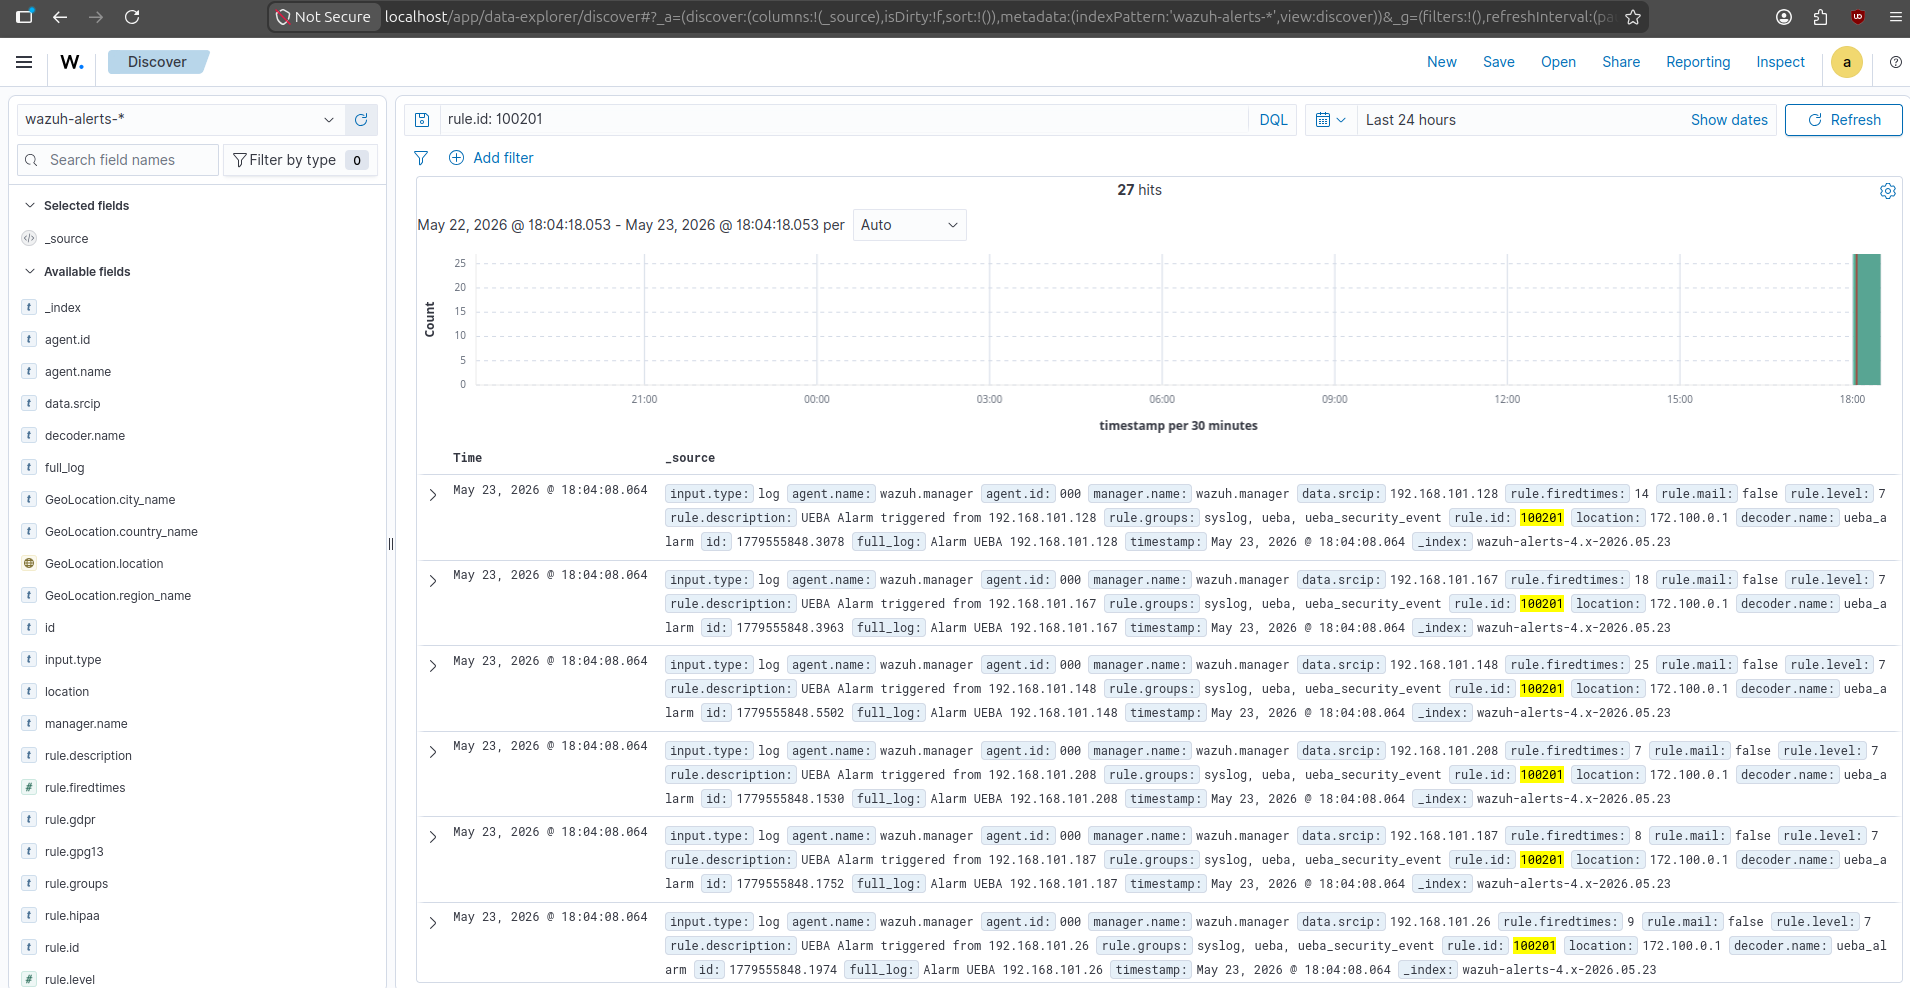
\includegraphics[width=\textwidth]{Wazuh_dashboard.png}
\end{figure}

\hypertarget{conclusion}{%
\subsection{Conclusion}\label{conclusion}}

The UEBA module identified 31 anomalous devices (21 internal and 10
external) across nine distinct behavioural patterns in the test
period. Every threshold was derived exclusively from the training
dataset, ensuring that no test-period information influenced the
baselines and that each detection reflects a genuine deviation from
established normal behaviour.

The pipeline demonstrates that a small set of complementary statistical
rules, each measuring a different dimension of behaviour, can cover a
broad threat surface without redundancy. Cumulative upload volume catches
both bulk and low-and-slow exfiltration; timing regularity exposes
botnet implants that leave no volumetric footprint; geographic and
infrastructure novelty flags coordinated reconnaissance campaigns; and
set-membership checks catch rogue devices that deliberately stay below
every volume threshold.

The seven HIGH-confidence detections, each corroborated by two or more
independent rules measuring entirely different signals, represent the
strongest candidates for immediate escalation. The 24 MEDIUM-confidence
detections provide a prioritised triage list where every alert carries
an explicit justification tied to a specific observed value and its
distance from the training baseline, giving an analyst the context
needed to make an informed decision rather than a bare IP address.

\end{document}
